%版权信息:王奥
\documentclass[UTF8]{ctexart}
\usepackage{ctex}
\usepackage{url}
\usepackage{cite}
\usepackage{graphicx}
\usepackage{wrapfig}
\title{中科大大一学生学习情况报告}
\author{田丽菲,王奥,罗靖宇}
\date{\today}

\begin{document}

\maketitle


\section{引言}
中国学生在大学以前往往是在父母老师的督促下学习,而以前师长们就不断和我们强调大学学习对自主性
的要求,来到大学后我们对此更是有了切身体会。大量研究和新闻表明,许多大学生存在各种各样的学习
问题
\paragraph*{(1)大量学生沉迷手机、电脑}
“我的一个同学,从大一到大四,四年的时间,除了考试和教室见个面,其他时间全部在寝室打游戏或者看武侠,反正大学里也没有人管。后来因为挂科太多被学院劝退,家长过来求情延缓时间,但于事无补,游戏照打不误,直到大四时无法毕业。”\cite{game}
\paragraph*{(2)存在拖延问题,往往在ddl之前几天才开始任务}
“大学是学生步入社会前的重要学习阶段,但是目前我国大学生群体中超过三成存在明显的学习拖延现象,
且这种现象在不同高校、区域以及专业之间并未发现显著差异"\cite{delay}
\paragraph*{(3)无法管控自我的生活,晚睡晚起,不去上课}
“在正式开始上课之后,我更加见识了大学里很多人是怎么样上课的:早晨上课铃响了之后有很多人穿着拖鞋边
吃早点慢悠悠地晃进教室,吃完早点后看看上面的老师,讲{}得没意思,于是爬着再补一觉。有的学生干脆一睡
不起,大学里有句话是这样流传的:“一觉醒来一看表十点了,继续睡到十一点半,起来连早点、中饭一起吃了
。”\\
晚上十一点后,应该是夜深人静、正值休息的时候,如果你此时走进大学里的男生寝室,你绝对可以看到他们
的夜生活才“刚刚开始”,打游戏、玩麻将或者是看武侠小说,好不热闹。鲜见一起读书、共同讨论人生智慧的
场景,相反可以看到很多的大学生去网吧包夜,或者在寝室联机打游戏,他们的日常交流沟通内容就是游戏,
以至于很多学生迫不得已,为了和同寝室的哥们“打成一片”而“学习”打游戏。游戏已经成为了大学里男生的主
要“学习内容”,而且不少人发奋用功地学习了四年。”\cite{game}
\paragraph*{(4)缺乏自主学习能力,无法跟上课程}
\paragraph{}
所以我们产生了了解科大大一同学学习现状的想法,希望了解自己的学习状态相对于科大其他同学如何,为今后
自己的学习规划提供借鉴。同时希望找出一些存在于自身或其他同学身上的问题,并提出针对这些问题的解决
方法,为未来铺平道路
\paragraph{}
开始我们的调查后我们遇到不少困难,但在老师和同学的支持下,整个团队的共同努力下我们还是完成了这次
调查


\section{调查过程}
\paragraph*{确定调查方案}
我们一开始是使用打算线上问卷去收集数据,但考虑到填线上问卷的同学会有更高的手机使用频率,可能会影
响样本的随机性。于是在大家的讨论下,我们决定发放线下问卷。同时考虑到其他地点比如图书馆可能会引入
其他变量,我们决定在宿舍发放问卷以保证样本的随机性。
\paragraph*{调查前的准备}
相较于线上问卷,线下问卷操作的难度不可同日而语。首先我们需要获得在寝室发放问卷的许可;其次如果过
度打扰到其他同学可能会被投诉。为了获得发放问卷的许可,我们多方询问与努力,最后终于获得校学生活动
中心许可,非常感谢过程中楼管老师在下班后还能抽出时间来指导我们。一开始我们打算敲门当面填写,但是
这可能会打扰到同学们的休息并且引起同学们的反感,对后续的回收工作不利,最后才想到贴门的办法,同时
第二天在回收,给各个时间段回到寝室的同学填写时间。同时,在老师的建议下,我们决定发放一些小礼物以
提高问卷的回收率。
\paragraph*{问卷发放回收}
在3月9号(周六)晚我们开始发放问卷,次日回收,统计人数后购买礼物,在3月17号完成了礼物的发放,最后
获得了83份有效问卷。完成了调查。


\section{数据结果}
具体问卷及结果参见附件,不在此报告展示


\section{数据分析}

\subsection{过往竞赛学习}
\begin{wrapfigure}{1}[1cm]{0pt}
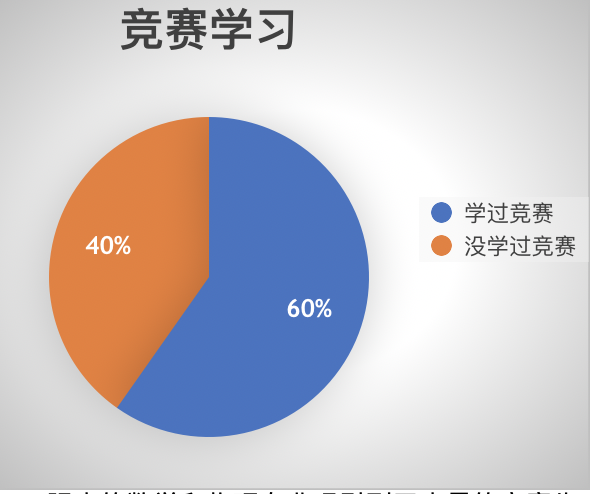
\includegraphics[width=5cm]{chart/竞赛学习.png}
\end{wrapfigure}
在被调查的新生中,有60\%的同学学习过竞赛,占被调查者中的大部分,40\%未学习过竞赛。这充分体现了科
大的理科实力,以其强大的数学和物理专业吸引到了大量的竞赛生,也侧面反映了科大对竞赛生招生的一定倾
斜。而在这方面,性别几乎未体现出差异,大大出乎我们的意料。但可能存在对学习过竞赛界定不清的情况:
可能有同学只是对竞赛有所接触就选择了学习过竞赛,如果把自招进入科大作为竞赛最低标准的话,这个比例
显然远高于实际,但是即使如此依然反映了科大同学即使在应试教育下依然有探索未知的好奇心,我想这也是
我们聚集在科大的原因.

\subsection{学习时间情况}
\paragraph{}
在被调查者中,有69\%的学生工作日的日均学习时间超过了3小时。即使在周末仍有46\%的同学学习时间周末
日均学习时间超过了3小时。这表明科大的大一同学们自律性较强,可以很好地把握自己的学习时间。令人感
兴趣的是在这个方面,性别带来了明显的差异。在接受调查的18位女生中有13位女生的工作日日均学习时间
超过了4小时,而在65位男生中只有25位日均学习时间超过了4小时。然而经过我们的大致估算,男生的周末
日均学习时间的平均值超过了7.2小时,而女生的周末日均学习时间却仅仅超过5.5小时。\\
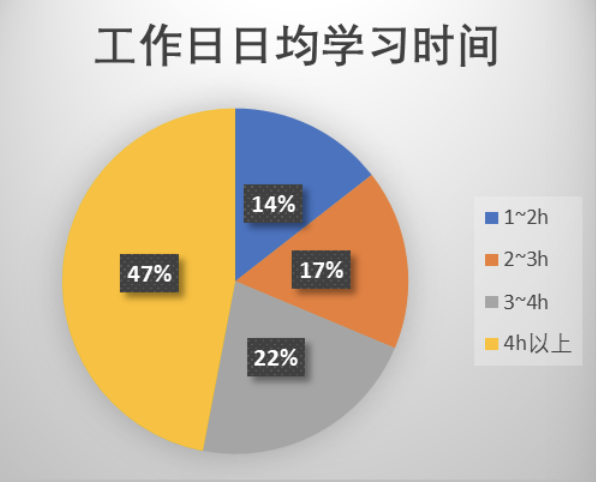
\includegraphics[height=5cm]{chart/工作日日均.png}
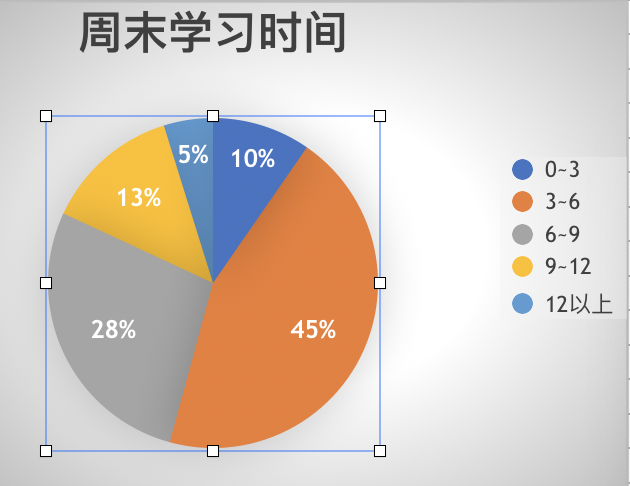
\includegraphics[height=5cm]{chart/周末.png}
\paragraph{}
我们觉得出现这种差异的直接原因男女生性格差异。很多研究发现了性别对于学习情况的影响,诸如:
\subparagraph*{}
\textbf{大学生手机依赖总分及失控性因子在性别上存在显著的差异\cite{phone}}
\subparagraph*{}
\textbf{相对男生来说,更高比例的女生认为有必要在 上新课前对学习的知识点进行提问复习,而且全勤
的女生比例达到86.32\%,高于男生 21.43\%,表明大学女生的学习态度更好,同时具有更强的主动学习动
机。\cite{genderdifference}}
\subparagraph*{}
\textbf{表4显示,大学生学习拖延总体上不存在性别差异。但在完成作业方面,男女生之间有极显著差异,
男生学习拖延程度显著高于女生;在学习拖延对情绪的困扰方面, 男女生之间也存在极显著差异, 学习拖延
给男生造成的情绪困扰明显低于女生\cite{delay}。}
\subparagraph*{}
我们觉得女生倾向于内敛、细腻的性格特征决定了她们在学习期间,能够保持良好的耐性与自律性,同时由于
拖延会带给他们更大的困扰,她们更倾向于在工作日完成学习任务,而文献[2]指出大学生群体中女生在手机
依赖总分、戒断性、失控性、低效性的得分上显著高于男生,尤其是在失控性上。而男生在逃避性上得分高于
女生\cite{phone}。此结论虽然有点出乎意料,但它很好地解释了女生在周末学习时间较少的现象。
\subparagraph*{}
我们认为男生更好动的性格特征让男生更难静下心来学习。同时男生的娱乐很大部分是可以碎片化完成的,例
如游戏和者体育运动等等,这些碎片化的娱乐不会占用周末的大部分时间,而工作日时间却会被碎片化的娱乐
项目分割。而女生通常都不太喜爱游戏或体育运动,娱乐项目大多需要集中的时间,例如追剧和购物等等,这
直接导致女生的娱乐项目集中在周末,降低了女生在周末的学习时间,也使女生在工作日基本投入学习当中。
与之相应,男生的作业会相对堆积到周末,交作业的压力会迫使他们在周末更多地投入时间。

\subsection{课余活动}
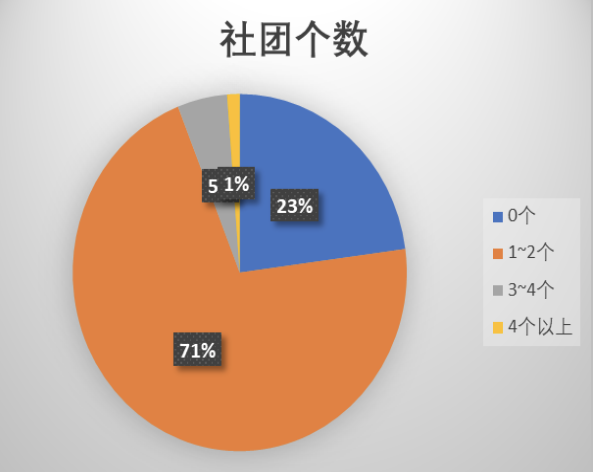
\includegraphics[height=5cm]{chart/社团个数.png}
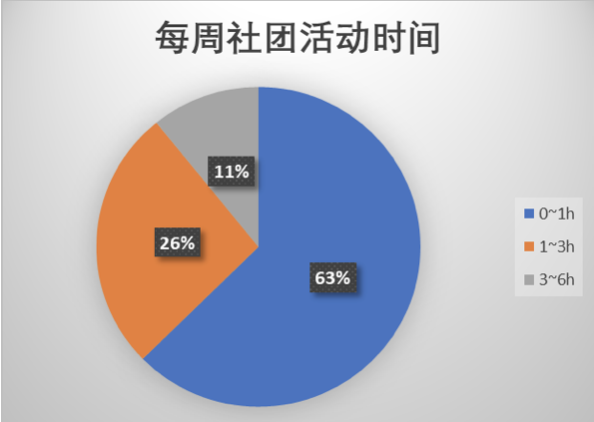
\includegraphics[height=5cm]{chart/每周社团活动时间.png}
在被调查者中,有23\%的人未参与任何社团活动。71\%的学生只加入了1~2个社团。有63\%的学生每周社团
活动时间只有0~1小时,仅有11\%的学生社团活动时间超过了3小时。这些无不体现了学生们对社团活动的热
情程度并不高。事实上,这反映了科大同学在学习之外能力的缺失。从4.2的结果中我们可以看出科大同学把
大量时间花于学习,严重的挤压了其他活动的时间。这固然表现了科大浓厚的学习氛围————”可以放下一张安
静的书桌“,但生活重心单一化容易导致稍有意外便陷入迷茫。虽然学校和学院举办了各式各样的课余活动,
诸如“越野跑“、文艺活动、野外实习,并且在社团建设上给予了很大的关注和支持,但繁重的学业负担,积重
难返的学习氛围,以及部分同学沉迷手机、窝在寝室。科大学生的课余生活仍然被频繁吐槽。就我个人而言,
基本不会参加那种文艺活动。同时可能学生都忙着自己的学习并适应大学新的教学方法,没有过多的时间去参
加一些社团活动。

\subsection{生活满意程度}
\begin{wrapfigure}{1}[1cm]{0pt}
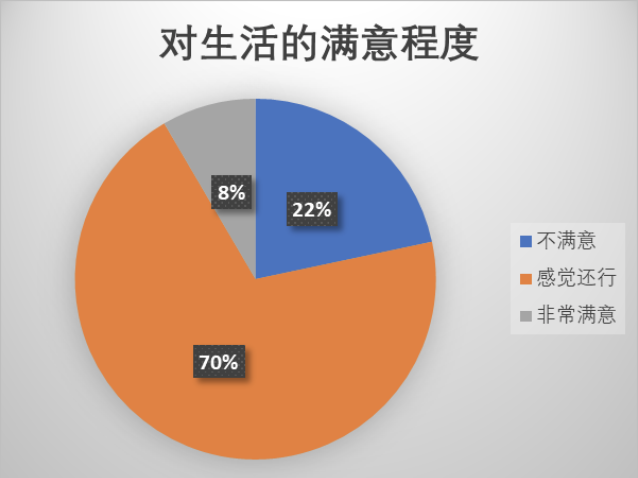
\includegraphics[width=5cm]{chart/生活满意程度.png}
\end{wrapfigure}
在被调查者中,有22\%的人对自己的生活感到不满意。我们觉得这个比例还是有点高。我们认为有两个方面的
原因。
\paragraph{(1)}科大的的基础教育一向走在国内前列,所以可能对学生的要求较高,有一些学生无法达到高
要求也是正常的事情。而且科大这个集体里都是经过高考选拔出来的精英,进入科大之后面临的激烈的竞争带来
的落差难免会让他们有所不适。而科大同学大部分对自己有较高的要求,而大学和中学学习方法存在较大差别,
这种不适应带来的压力和工作量会导致让他们身心俱疲。难免产生不满。
\paragraph{(2)}科大注重理科教育,对数理基础的要求与部分同学的专业预期不符。同时许多同学对自己的
专业不太满意(下文详述),也有些同学对自己的未来比较迷茫,觉得科大过分注重科研不适合自己,也有的同学
觉得科大基础设施不完善。这也是导致不满的原因

\subsection{专业选择}
\begin{wrapfigure}{1}[1cm]{0pt}
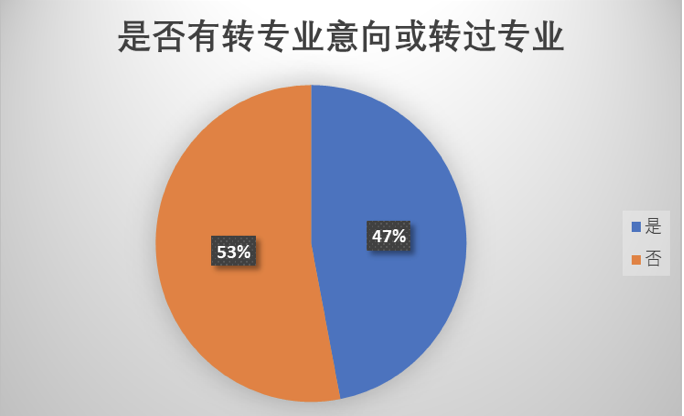
\includegraphics[width=5cm]{chart/转专业.png}
\end{wrapfigure}
在被调查者中,47\%的人有转专业意向或已转过专业,占有相当的比例。我们认为出现这类现象的原因是我们
当初选择专业时并不了解专业,而且有大量同学是被调剂的。这个结果反映了科大宽松的专业选择制度的必要
性,由于科大在大一安排的课大多是通修的基础课,所以课程对于专业选择方面的限制较小。而科大原则上对
所有学生的专业选择没有限制,使得同学可以在经历了大学一年的了解后作出自己的选择,有利于同学未来的
发展

\subsection{学习动力}
\begin{wrapfigure}{1}[1cm]{0pt}
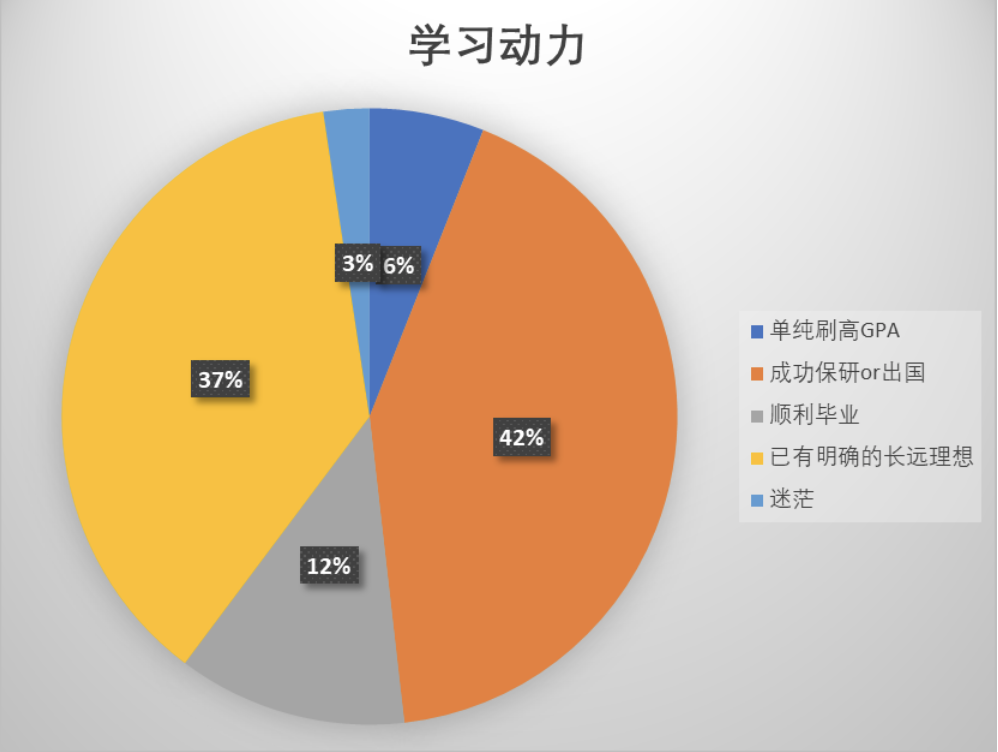
\includegraphics[width=5cm]{chart/学习动力.png}
\end{wrapfigure}
在学习动力的的调查上我们发现科大学生有37\%是已有明确长远目标并为之奋斗的,这个比例远高于我们的预
期。“而当代大学生的近景性动机过多, 为了报恩,为了找到好工作,为了高收入等等,具有直接性、短期性,有明
显的功利性目的;只有两项(序号6“发展自己、完善自我”,序号13“证明我的价值和能力”)能体现远景性学习动
机, 而且比例也不高,分别为49.2\%和45.8\%。还通过与大学生直接谈话再了解他们远景性动机 ,绝大多数学
生首先还是考虑就业 ,他们认为在现在竞争如此激烈的社会首先要考虑生存 ,其他的所谓“理想、信念、抱负
”还没时间去想,可见,当代大学生的远景性动机明显不足"\cite{learninggoal}。”说明科大学生相较于其
他同龄人对自己的未来有着高远的目标,而且我们注意到这类同学往往投入学习的时间更多,生活满意度更高,
且从收集到的少部分的GPA来看,他们的学习成绩高于其他。但我们依然要注意那12\%只求顺利毕业,6\%的
单纯刷高GPA和3\%的迷茫的同学。身为刚进入大学的学生,便只求毕业,失去了锐气,这无疑是不正常的,而
且我们认为这样反而可能无法顺利毕业。而单纯刷高GPA的同学的心态也存在问题,我觉得这就是科大这种学
习氛围的副作用,我觉得我们需要明白,GPA不是全部,还要注重发展其他方面的能力。至于剩下那3\%的同学
应主动寻找学习的意义,学校也应该组织帮助他们。

\subsection{对数据及分析的反思}
\paragraph{}事实上,由于经验不足,我们的问卷和分析存在不少缺陷。例如问卷可能存在歧义,反映了我们考虑的局限性。
这让我们体会的了科研调查的不易,让我们对在正式问卷前应进行试调查的必要性有了更深的体会。
\paragraph{}
同时问卷由于数据数量以及分析手段的限制,对于一些数据的关联性不好进行分析。要调查相关数据可能需要更
大的样本数目,但即使是对当前数目的样本进行分析都存在一定困难。可能在我们掌握相关计算机知识后会更加
方便。同时我们缺乏分析三个及以上因素的综合关联的能力。导致结果差强人意。让我们了解了科研对于各方面
的能力都有要求,今后学习中应加强培养相关的能力。


\section{总结}
支持问卷调查让我们初步认识了科研的过程,同时对科大学生的学习情况有所了解.以下为我们总结的经验教训
\paragraph{长远理想}
应结合自身实际,树立可行有意义的理想.现代大学生普遍缺乏远景性学习动机,原因有(1)缺乏挫折体验,知难
而退;(2)就业的过大压力, 削减了学生的学习热情;(3)社会缺乏有效的信念引导;(4)价值观物质化、功利化
、眼前化,信念的淡化\cite{learninggoal}。 豪·厄尔和沃森的研究则表明,大学生学习拖延与内在学习动机
显著负相关\cite{delay}。那些有着远大理想的同学往往有着更好的学习习惯。
\paragraph{坚持初心}
虽然我们只调查了大一的同学,同学们成绩(可能有成绩差的同学倾向于不提供GPA的因素普遍不差。但以我们个
人及老师的体会及而言,经过半个学期,同学们学习的动力有所衰退。研究也表明学习习惯与年纪城明显的反相关
:大一学生的作业拖延明显低于其他年级;大二学生的作业拖延显著高于大一学生,但与大三、大四学生无显著差异。
在学习拖延对情绪的影响方面,大一到大四呈逐年降低趋势;大一学生与大三、大四学生有显著差异, 拖延对大一
学生造成的情绪困扰明显高于大三、大四学生;学习拖延给大二学生造成的情绪困扰也显著高于大四学生\cite{
delay}。所以同学们要努力保持大一的学习状态,这样顺利毕业必然不成问题。而我觉得有理想者更容易保持初心
。
\paragraph{远离手机、电脑}
”大学生手机依赖与学业拖延及各因子分呈显著正相关“\cite{phone},“大学生由于存在不同程度的手机依赖
现象,在他们沉迷手机的同时占据了完成学业任务的时间。也有部分大学生在 完成学业任务的中途遇到难点不能
攻克,或是对学业任务有点厌烦时,都会掏出手机借此逃离学业的任 务。但是在完成学业任务时一旦停止,再重
新进入状态是需要一段时间的。这个无形中其实也浪费了学 习时间,拖延了学业任务的完成时间。反过来,大学
生的学业拖延行为又会进一步增加手机依赖现象。”\cite{phone}
\paragraph{走向户外}
无论是沉迷于学习或是肥宅于寝室都是不可取的,沉迷于学习会使生活容易失去重心。而老师学长也一再强调不要
一直呆在寝室。那会使人失去进取的动力,同时在寝室学习更难集中注意力。容易让人学着学着就到床上去了。
参加课余活动可以培养我们其他方面的能力,同时给我们以人文熏陶。我想这也是学校身为一个理工科院校却经常
举办文艺活动的原因。

\section{致谢}
感谢学校对新生研讨课的支持。感谢为本调研提供帮助的教师,宿管阿姨。感谢所有参与问卷调查的同学!

\bibliographystyle{plain}
\bibliography{docu/docm}
\end{document}